% 1. ročník MAT – příprava 98; inspirace Realisticky.cz 020501–020506, úlohy nově sestavené.
\documentclass[11pt,a4paper]{article}
\input{../../sablony/pripravy/priprava.sty}
\usepackage{tikz}
\usepackage{pgfplots}
\pgfplotsset{compat=1.18}
\usetikzlibrary{arrows.meta}
\nastavPripravu{1. ročník}{Kvadratické funkce}{98}{Posuny paraboly a vrcholový tvar}
\begin{document}
\blok{Posouváme známý graf}
Připomeňme si posuny přímek a grafů s absolutní hodnotou. Stejná pravidla fungují u paraboly: změna \emph{uvnitř závorky} posouvá vodorovně, číslo \emph{mimo závorku} svisle. Pro $x=m$ je výraz $(x-m)^2$ nulový.
\begin{definiceBox}
\textbf{Vrcholový tvar} kvadratické funkce je
\[ f(x)=a(x-m)^2+n,\qquad a\ne0.\]
Vrchol je $V[m;n]$, osa souměrnosti má rovnici $x=m$.
Je-li $a>0$, pak $H(f)=\langle n;+\infty)$; je-li $a<0$, pak $H(f)=(-\infty;n\rangle$.
\end{definiceBox}
\begin{center}
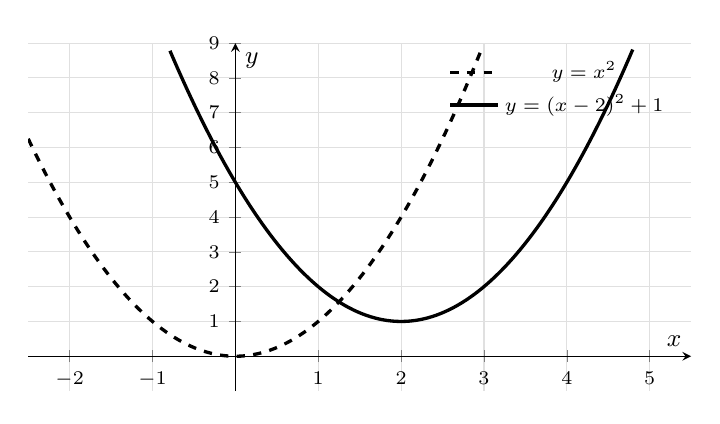
\begin{tikzpicture}
\begin{axis}[
width=10cm,height=6.0cm,axis lines=middle,
xmin=-2.5,xmax=5.5,ymin=-1,ymax=9,
xtick={-2,-1,...,5},ytick={0,1,...,9},grid=both,
minor tick num=0,grid style={black!12},
tick label style={font=\scriptsize},xlabel={$x$},ylabel={$y$},
label style={font=\small},restrict y to domain=-1:9,
clip=true,legend style={font=\scriptsize,draw=none,fill=none,at={(0.98,0.98)},anchor=north east},
]
\addplot[very thick,dashed,domain=-2.5:5.5,samples=160] {x^2};
\addlegendentry{$y=x^2$}
\addplot[very thick,solid,domain=-2.5:5.5,samples=160] {(x-2)^2+1};
\addlegendentry{$y=(x-2)^2+1$}
\end{axis}
\end{tikzpicture}
\end{center}
\blok{Společně řešené příklady}

\begin{prikladReseniBox}
Vyznačte vrchol, osu, obor hodnot a posun u $f(x)=(x-2)^2+1$. Vypočtěte dva body souměrné podle osy paraboly.
\tcblower
\[
\begin{aligned}
V&=[2;1],\quad\text{osa: }x=2 \\
H(f)&=\langle1;+\infty) \\
f(1)&=2=f(3) \\
A&=[1;2],\quad B=[3;2]
\end{aligned}
\]
Parabola vznikne posunem $y=x^2$ o dvě doprava a jednu nahoru.
\end{prikladReseniBox}
\begin{prikladReseniBox}
Určete vlastnosti $g(x)=-2(x+1)^2+3$. Rozhodněte, zda má maximum nebo minimum.
\tcblower
\[
\begin{aligned}
g(x)&=-2(x-(-1))^2+3 \\
V&=[-1;3],\quad \text{osa: }x=-1 \\
H(g)&=(-\infty;3\rangle,\quad \max g=3 \\
g(0)&=-2+3=1
\end{aligned}
\]

\end{prikladReseniBox}
\blok{Samostatné procvičování}

\begin{zadaniReseniBox}
a) Pro $p(x)=(x+3)^2-2$ určete vrchol a osu.\par
b) U $q(x)=\tfrac12(x-4)^2-1$ určete obor hodnot a souřadnice průsečíku s osou $y$.\par
c) Sestavte předpis paraboly vzniklé posunem $y=-x^2$ o 2 doleva a 5 nahoru.
\tcblower
\[
\begin{aligned}
V_p&=[-3;-2],\quad \text{osa }x=-3 \\
H(q)&=\langle-1;+\infty),\quad q(0)=7 \\
r(x)&=-(x+2)^2+5
\end{aligned}
\]

\end{zadaniReseniBox}
\blok{Volitelná rezerva}
Na omezeném definičním oboru $D=\langle0;2\rangle$ zkoumejte $f(x)=(x-3)^2+1$. Vrchol $x=3$ leží mimo zadaný obor; proto minimum na $D$ není $1$, nýbrž $f(2)=2$. Maximum je $f(0)=10$.
\blok{Domácí úkol}
\begin{zadaniReseniBox}[title={Domácí příprava}]
\begin{enumerate}[label=\alph*),itemsep=3pt]
\item Určete vrchol a osu souměrnosti $f(x)=(x-4)^2+2$.
\item Určete vrchol, maximum nebo minimum a $H(g)$ pro $g(x)=-(x+2)^2+5$.
\item Vypočtěte $h(-1)$, $h(1)$ a $h(3)$ pro $h(x)=2(x-1)^2-3$.
\item Zapište předpis posunu paraboly $y=x^2$ o 3 vlevo a 4 dolů.
\item Určete $a,m,n$ v předpisu $f(x)=-\frac12(x-2)^2+1$; určete $H(f)$.
\item Naskicujte $y=(x-1)^2-2$ pomocí vrcholu a čtyř bodů souměrných podle osy.
\item \textbf{Výzva:} Pro $f(x)=(x-3)^2+1$ a $D(f)=\langle0;2\rangle$ určete obor hodnot.
\end{enumerate}
\tcblower
\begin{enumerate}[label=\alph*),itemsep=4pt]
\item
\[
\begin{aligned}
V&=[4;2],\quad\text{osa }x=4
\end{aligned}
\]

\item
\[
\begin{aligned}
V&=[-2;5],\quad\max g=5 \\
H(g)&=(-\infty;5\rangle
\end{aligned}
\]

\item
\[
\begin{aligned}
h(-1)&=5,\quad h(1)=-3,\quad h(3)=5
\end{aligned}
\]

\item
\[
\begin{aligned}
f(x)&=(x+3)^2-4
\end{aligned}
\]

\item
\[
\begin{aligned}
a&=-\tfrac12,\quad m=2,\quad n=1 \\
H(f)&=(-\infty;1\rangle
\end{aligned}
\]

\item
\[
\begin{aligned}
V&=[1;-2],\quad [0;-1],\ [2;-1] \\
[-1;2],&\quad[3;2]
\end{aligned}
\]

\item
\[
\begin{aligned}
f(2)&=2,\qquad f(0)=10 \\
H(f)&=\langle2;10\rangle
\end{aligned}
\]

\end{enumerate}
\end{zadaniReseniBox}
\poznamka{Čas: motivace 5 min, dva příklady 15 min, společný graf 8 min, samostatně 12 min, shrnutí 5 min. Zdůrazni, že ve tvaru $(x+3)^2$ je vrchol při $x=-3$, nikoli při $+3$.}
\end{document}
